
%----------------------------------------------------------------------------------------
%	PACKAGES AND OTHER DOCUMENT CONFIGURATIONS
%----------------------------------------------------------------------------------------

\documentclass[12pt]{report}
\usepackage[english]{babel}
\usepackage[utf8x]{inputenc}
\usepackage{amsmath}
\usepackage{graphicx}
\usepackage{float}
\usepackage[colorinlistoftodos]{todonotes}
\usepackage{cite}
\usepackage{url}
\usepackage[margin=1in]{geometry}


\begin{document}

\begin{titlepage}

\newcommand{\HRule}{\rule{\linewidth}{0.5mm}} % Defines a new command for the horizontal lines, change thickness here

\center % Center everything on the page
 

%%	HEADING SECTIONS  %%

\textsc{\LARGE Imperial College London}\\[1.5cm] % Name of your university/college



%%	TITLE SECTION  %%


\HRule \\[0.4cm]
{ \huge \bfseries Smart Rods (Hardware) \\ Interim Report}\\[0.4cm] % Title of your document
\HRule \\[1.5cm]
 

%%	AUTHOR SECTION  %%


\begin{minipage}{0.4\textwidth}
\begin{flushleft} \large
\emph{Author:}\\
Mattin \textsc{Mir-Tahmasebi} % Your name
CID: 00824754
\end{flushleft}
\end{minipage}
~
\begin{minipage}{0.4\textwidth}
\begin{flushright} \large
\emph{Supervisor:} \\
Prof. George \textsc{Constantinides} % Supervisor's Name
\end{flushright}
\end{minipage}\\[2cm]

% If you don't want a supervisor, uncomment the two lines below and remove the section above
%\Large \emph{Author:}\\
%John \textsc{Smith}\\[3cm] % Your name



%%	LOGO SECTION  %%



\includegraphics[width=0.5\textwidth]{ImperialCrest.jpg}\\[1cm] % Include a department/university logo - this will require the graphicx package
 
%----------------------------------------------------------------------------------------

\vfill % Fill the rest of the page with whitespace

\end{titlepage}

%% ACKNOWLEDGEMENTS  %%

%% ABSTRACT %%

\pagenumbering{roman}

\begin{abstract}
Your abstract.
\end{abstract}
\newpage

%% CONTENTS %%

\tableofcontents
\thispagestyle{empty}
\newpage


\pagenumbering{arabic}
\setcounter{page}{1}


%% CHAPTERS %%

\chapter{Project Specification}



Cuisenaire\textsuperscript{\textregistered} Rods \cite{TheCuise14:online} are an educational tool used in primary school mathematics classes to aid in the learning of 'number bonds'. These are simple addition sums typically resulting in a round number like 10 or 20, such as $7+3=10$, which children learn as a foundation for more complex mathematical relationships. These are an important part of the Key Stage One (ages 5-7) curriculum in the UK, as recommended by the British Government \cite{Mathemat26:online}. 

\begin{figure}[h] 
  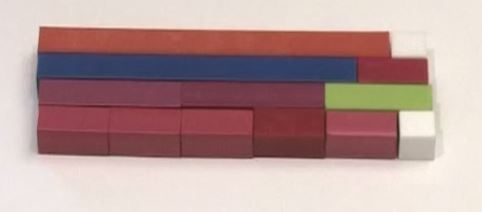
\includegraphics[width=0.75\textwidth]{rods.JPG}
  \centering
  \caption{A set of Cuisenaire\textsuperscript{\textregistered} Rods in use \cite{24Lesnom77:online}}
  \label{fig:rods}
\end{figure}

A set of rods consists of different-coloured cuboids, each of a different length, the smallest of which represents one unit. The rest of the rods are sized in multiples of this unit up to the longest rod, usually of size 10. Pupils are taught how different sized rods can be placed to end-to-end in order to reach the target summation result, and are encouraged to find several alternate combinations of rods that add to the result, as demonstrated in Figure \ref{fig:rods}. This is a physical representation of number bonds, as the pupil can associate a 7-rod (a rod of length 7) and a 3-rod forming a line of length 10 units with the mathematical fact that $7+3=10$. \\

The current disadvantage of the use of these rods is that in a class of dozens of students, it can be difficult for a teacher to monitor and track student progress. The teacher can survey the classroom, but is not capable of giving every student constant attentions, so inevitably, poor progress sometimes goes unnoticed and students may fall behind without extra support. The aim of this project is to design and build a product that resolves this, by using a technologically-enhanced version of the rods which will allow the teacher to detect struggling pupils and provide assistance to them. They should do so by gathering data about the way the students are using the enhanced rods, such as time spent forming a number bond, how many combinations were found, and perhaps even more complex information like detecting patterns in which solutions were discovered. This data can be analysed to provide an overview of how the entire class is coping with the task.\\

The project is split into two halves: the software, including processing of data and user interfaces, is being completed by another student (Pierre Azalbert). The hardware, including the design and production of the rods, is the focus of this report.\\

Making the correct design choices will greatly affect the efficacy of the product. The final product will likely be used by publicly-funded schools, so costs should be kept low. The aim of the product is to make the teaching process easier for the teacher and to improve the learning experience for the pupils, so care should be taken to make the product as accessible as possible for both parties. This means keeping setup steps simple for teachers, and using human-computer interface (HCI) principles to ensure students find the product easy to use.

\chapter{Background}

\section{Cuisenaire\textsuperscript{\textregistered} Philosophy}
Background research began with discovering how Cuisenaire\textsuperscript{\textregistered} rods are used and why they are useful. John V. Trivett, in his article, \emph{The Cuisenaire Rods—Numbers in Colour}, from the Journal of the Association of Teachers of Mathematics \cite{johnv.trivett1962} talks about how abstracting the notation from the teaching of mathematics allows students to form conceptual instincts about ratios between values. He argues this is more valuable than committing equations and expressions to memory to be regurgitated during examinations. This idea is reinforced by Tony Wing in his article in the same journal, \emph{Working Towards Mental Arithmetic... And (Still) Counting}\cite{tonywing1996}, where he states that it is important for children to learn to play with the rods \say{before conventional number names and symbols are attached to them}.\\

This is something to keep in mind throughout the design process: we want to adhere to that principle of abstraction and not construct the rods in a way that would cause the children to treat them as numbers, for example, by having each rod's length written on it. \\

\section{Teacher Advice}

Further research was carried out by contacting primary school maths teachers who have made use of Cuisenaire\textsuperscript{\textregistered} rods, to ask them about the benefits of the rods and what could be improved. A criticism of the rods is that teachers need to record proof of students' work for administrative purposes, and the rods do not lend themselves to this very well because the children are required to draw diagrams of their solutions in workbooks, which takes considerable time from the exercise. This is a problem that our product will likely be able to solve, as an electronic system will be able to record every attempt a student makes at an answer, meaning that our records will be more detailed than what the children could draw themselves.\\

Another complaint was that, often, neither students nor teachers know how to properly make use of the rods when presented with them. This creates, for us, a task in human-computer interaction, as we will have to design a system that is intuitive to use with little mental effort required by the user. This includes being intuitive to set up (for teachers) and intuitive to operate (for children).\\

It was warned that students may not treat the product with care and so it should be able to withstand bending or general mistreatment at the hands of the children. This will inform our choice of material and construction method once we begin production. \\


\section{Similar Products}
Online searching yielded very few internet-enabled educational devices for the KS1 demographic, excluding educational applications for tablets and computers. This means that we will not be able to compare the hardware aspect of our product to existing designs, and will be setting precedents with some of our design choices. While this gives us the opportunity to explore and discover new methods of integrating technology into teaching, it does mean that the chance of our ideas being unsuccessful are increased, as we do not have a foundation of work to build upon. This effect can be mitigated via consultation of our contacts in schools and by working closely with our supervisor who can help guide our path.





\chapter{Design Choices}


\section{Where should electronic complexity lie?}
\label{sec:complexity}

Some form of electronic device has to be used to identify the relative positions of the rods, but we have some choice in where this device exists. If we want to keep our product to be simply a set of rods, then the only place for the device is within the rods themselves. The rods would each need to be able to communicate with each other, to discern relative position, and also with either a controller that relays messages to the server or to the server directly.\\

Unfortunately, this solution brings several impracticalities. Firstly, the size of the rods has to be kept small, which constrains the size of battery we could embed into them. They will have to be capable of transmitting and receiving wireless messages, and even perhaps perform some amount of processing, so their power consumption will be too high for a battery of that size. Charging the batteries would also be impracticable; consider a classroom of around 30 students, each with a set of dozens of rods, and it becomes clear that the hassle of having to charge each device individually would outweigh any benefit of the product to a teacher.\\

Another issue concerns the identification of rods and their assignment to students: remember again that each student needs their own set of dozens of rods, and that any information these rods transmit will be attached to that child’s profile. The teacher would have to perform the frustrating and repetitive task of assigning each rod to a student, causing a considerable amount of inconvenience. Additionally, we must keep in mind that our target users are children, who may have the tendency to take rods from another student, misplace their own rods, or perhaps even throw rods around the classroom – all of these actions could cause sets of rods to be mixed together, leading to incorrect data being sent to the server, as progress from one student will be attached to the profile of another.\\

The last issue is economic: each of these rods will require several electronic components, including a processing unit and wireless transceivers, driving the cost of each unit up considerably. This is especially relevant as the smaller rods are easily lost in the classroom, so replacements would likely need to be purchased, increasing ongoing costs further.\\

An alternative solution to putting complexity in the rods is to design a playing board with which the rods can interact, and embed the majority of the electronics in that instead. The 10x10 board would resemble a chess board, with grid squares guiding the placement of rods. The students arrange their rods on the board, which can identify the positions of the rods through some means, and communicate that data to the server. This alleviates all of the problems detailed above. The board is large and can house a larger battery than the rods, so there would be no power problem. There would only be one board per child so there are fewer devices to charge and much less work involved in assigning devices to children, also meaning that mixing of rods is not an issue, as it is the board which is unique to the child, not the rods. The cost to replace rods would be much lower as they would not contain as much electronics, and the overall cost would be lower as only the boards would require processing and communications equipment, as opposed to fitting one to every rod.\\ 

During an interview with a primary school teacher, we were informed that having a board may actually aid in the students’ learning, as having a grid could help them conceptualise how the rods fit together. 

\section{How should the board detect rod positions?}
\label{sec:detection}  


Having settled on the use of a board, the next design choice to be made is what technology it will make use of to detect where rods have been placed. The chosen method needs to have the following characteristics to be viable: it must be able to \textit{reliably} detect rods and their positions, as any errors may mislead and confuse the child, weakening the product’s effectiveness as an educational tool. It should keep \textit{cost} low, as there could be up to hundreds of these products in use at an institution, and since they will likely be using public funding they will be under budget constraints. It should keep \textit{power consumption} to a minimum to maximise the amount of use between charges. Lastly, it should remove as much \textit{complexity} from the rods as possible, for the reasons outlined in section \ref{sec:complexity}.\\

%%  Weight %%

\subsection{Weight}
\label{weight}

Rods could be given different weights, which are sensed by load sensors on the board. Each weight would be mapped to a different length of rod.\\

{
\setlength{\parindent}{0pt} % Remove paragraph indents within this block

\textbf{\textit{Reliability:}} It may be difficult to distinguish between the weight of a rod and the weight from the child touching the board, which could lead to false readings. However, under good conditions it should be possible to distinguish between rods well.\\

\textbf{\textit{Cost:}} The cost of the rods will likely be low, as they will just require weighting, however the board will require a load sensor in every grid square. The load sensor would need to be small enough to fit into a square around $2cm^2$ in area, and be sensitive enough to detect weighted rods light enough for a child to safely play with. A preliminary search revealed that components meeting those specifications would cost tens of pounds  \cite{ref:loadsensor}. Considering we are using a 10x10 board, purchasing 100 of these components would increase the cost to unacceptable levels.    \\

\textbf{\textit{Power Consumption:}} The datasheet of a suitable sensor \cite{MICROSWI18:online} states a typical voltage requirement of $10V$, and an input resistance of $5k\Omega$. Using $P=\frac{V^2}{R}$ we can determine a power usage of $0.02W$. 100 of these components would then draw 2W. \\

\textbf{\textit{Rod Complexity:}} The rods will not need any electronics, just some weighted material, so the complexity is quite low.\\
}

%%  Magnets %%

\subsection{Magnetic Fields}
\label{magnets}

Magnets of varying strength could be inserted into rods to be detected by magnetometers/gaussmeters in the board. Each strength would be mapped to a different length of rod. \\

{
\setlength{\parindent}{0pt} 

\textbf{\textit{Reliability:}} This method would likely prove to be quite unreliable, due to the close proximity of each of the grid squares - a magnetic field emanating from a rod \\

\textbf{\textit{Cost:}}\\

\textbf{\textit{Power Consumption:}}\\

\textbf{\textit{Rod Complexity:}}\\
}

%%  RFID %%

\subsection{RFID}
\label{rfid}

Passive RFID chips could be inserted into the rods, and RFID sensors into the board. Each RFID chip would contain identifying information about the rod it is in. When a rod is placed on the board, its RFID chip is powered and the data is read, and sent to the server. \\

{
\setlength{\parindent}{0pt} 

\textbf{\textit{Reliability:}} Our requirements are such that the range of detection of a rod should be very small, no more than a centimetre or so, as otherwise neighbouring grid squares could erroneously detect nearby rods and send false data to the server. A search for RFID products that operate in this range found no suitable results, which indicates RFID is not tailored to the precision detection needed for this project.\\

\textbf{\textit{Cost:}} An example of one of the shortest range components of the correct dimensions retails at between £5-14 per unit \cite{RITRPR9U23:online}; while this is much cheaper than the load sensor described above, it would still raise the price of the product to an unacceptable level given the quantity of boards/rods needed for a classroom.\\

\textbf{\textit{Power Consumption:}} Since the components in the rod are passive, they would draw a minimal amount of power \\

\textbf{\textit{Rod Complexity:}}\\
}


%%  RGB %%

\subsection{RGB Light}
\label{rgb}

Each grid square of the board could contain an RGB LED and a photodiode; the LED would flash periodically and the photodiode would measure the frequency of the reflected light. Since each rod is of a distinctly different colour, each would produce a different reflected frequency.\\

{
\setlength{\parindent}{0pt} 

\textbf{\textit{Reliability:}}\\

\textbf{\textit{Cost:}}\\

\textbf{\textit{Power Consumption:}}\\

\textbf{\textit{Rod Complexity:}}\\
}

%%  Resistors %%

\subsection{Shorting Resistor Chains}
\label{resistors}

Each row on the board could be linked by a long series chain of resistors of known values, and the rods themselves could contain a wire connecting two contact on either end of the rod. When the rod is placed on the board, its contacts would connect to contacts on the board, shorting a number of resistors in the board relative to the rod's length. The change in voltage at the different nodes in the line could be used to detect if and where a rod is placed.\\

{
\setlength{\parindent}{0pt} 

\textbf{\textit{Reliability:}}\\

\textbf{\textit{Cost:}}\\

\textbf{\textit{Power Consumption:}}\\

\textbf{\textit{Rod Complexity:}}\\
}


\chapter{Implementation Plan}


\chapter{Evaluation Plan}

The majority of the evaluation for this project is qualitative and subjective; the true judge of the success of the product will be the reactions of the teachers and students who will use the product. We will want to know if our design met our aim of helping teachers to keep a record of students' work, and to more easily track and monitor student progress, and also if it provides a friendly user experience for both teachers and students. \\

This should be achieved through communication with primary maths teachers, and visits to nearby schools where we can see how a classroom might make use of the product. We should observe the way in which the product is used, making note of unexpected ways in which the product is used or handled. Not being part of the target demographic for the product, it is likely there are some use-cases which we have not anticipated, and such instances would be taken into account if design for the product were to be continued further. The students should be monitored to see what, if any, frustrations they have with operating the product, and if they enjoyed using it. The teachers should be surveyed about the ease of set-up of the product (including charging and distribution among children) and about the merit the product has as an educational tool compared to other methods they have used. \\

The ideal evaluation would be a long-term study of a class using the product over the course of a year, along with a similar class using traditional rods or other methods of teaching, and comparing each class' performance and satisfaction over that year. This is, unfortunately, out of the scope of this project, so we have to settle with a much shorter-term survey. \\

Since this report focusses only on the hardware aspect of the product, evaluation considerations must focus on that aspect too. While it can be difficult to separate the concepts of software and hardware when trying to evaluate the product, one feature that is exclusive to the hardware is the reliability of rod placement detection. The accurate detection of rods is vital in ensuring children do not get confused when using the product, not only because it may cause them to misunderstand the lesson they are supposed to learn, but if they suspect the product does not function properly, they may be less inclined to engage with it in future. \\

To evaluate reliability, multiple possible configurations of rods should be tested and the response of the board should be recorded. The test should include extreme and edge cases, such as filling the entire board with rods, quickly placing and removing a rod, and adding many rods in quick succession. There is no margin of error, so every test needs to pass.





























\bibliography{references}
\bibliographystyle{ieeetr}

\end{document}